\documentclass{article}
\usepackage[utf8]{inputenc}
\usepackage[english]{babel} 
\usepackage{amsmath,amssymb,amsthm}
\allowdisplaybreaks[1]
\usepackage{hyperref}
\usepackage{pgfplots}
\usepackage{graphicx}
\usepackage{float}
\usepackage{fourier}

\newtheorem{theorem}{Theorem}[section]
\theoremstyle{definition}
\newtheorem{definition}{Definition}[theorem]
\newtheorem{corollary}{Corollary}[theorem]
\newtheorem{lemma}[theorem]{Lemma}

\newcommand{\plotSamples}{200}
\newcommand{\plotffprime}[2]{
	\begin{tikzpicture}
	\begin{axis}[
	axis lines*=middle,
	domain=-100:100,
	restrict y to domain=-20:20,
	samples=\plotSamples,
	ymin=-10, ymax=10,
	xmin=-10, xmax=10]
	\addplot[red] (x,{#1});
	\addplot[blue, dashed] (x,{#2});
	\legend{$f(x)$,$f'(x)$}
	\end{axis}
	\end{tikzpicture}
}
\newcommand{\plotffprimerange}[6]{
	\begin{tikzpicture}
	\begin{axis}[
	axis lines*=middle,
	domain=-100:100,
	restrict y to domain=-20:20,
	samples=\plotSamples,
	ymin=#5, ymax=#6,
	xmin=#3, xmax=#4]
	\addplot[red] (x,{#1});
	\addplot[blue, dashed] (x,{#2});
	\legend{$f(x)$,$f'(x)$}
	\end{axis}
	\end{tikzpicture}
}

\title{Calculus Handout}
\author{Daniel Frederico Lins Leite}
\date{September 2016}

\begin{document}
\section{Introduction}
\maketitle

\begin{theorem}[Squeeze theorem]\label{theorems:limits:squeeze}
	\begin{align*}
		\text{IF }& g(x) <= f(x) <= h(x)\\
		\text{AND }& \lim_{x->a} {g(x)} = \lim_{x->a} {h(x)} = L\\
		\text{THEN }& \lim_{x->a} {f(x)} = L
	\end{align*}
\end{theorem}
\paragraph{Used by:}
\begin{enumerate}
	\item {Theorem \ref{theorems:limits:sinxoverx}}
\end{enumerate}

\clearpage
\begin{theorem}[Limit of $sin(x)/x$]\label{theorems:limits:sinxoverx}
	\begin{align*}
	\lim_{x \to 0} \frac {sin(x)} {x} = 1
	\end{align*}
\end{theorem}
\begin{proof}	
	\text{Given that:}
	\begin{align*}
		\mu_1(\overline AB) = \text{LENGTH of } \overline AB\\
		\mu_2(\bigtriangleup ABC) = \text{AREA of } \bigtriangleup ABC
	\end{align*}
	\text{We have from the figure that:}
	\begin{align*}
		\mu_2(\bigtriangleup ACE) <= \mu_2( \widearc{ACE}) &<= \mu_2( \bigtriangleup ACD)\\
	\end{align*}
	\begin{figure}[H]
		\centering
		\includegraphics[scale=0.25]{images/limsinxoverx.eps}
	\end{figure}
	\begin{align*}
		\\
		\mu_2(\bigtriangleup ACE) &= \frac{1}{2} * \mu_1(\overline{AC}) * \mu_1(\overline{BE})\\
		\mu_2(\bigtriangleup ACE) &= \frac{1}{2} * 1 * \mu_1(\overline{BE})\\
		\mu_2(\bigtriangleup ACE) &= \frac{1}{2} * 1 * |sin(\theta)|\\		
		\mu_2(\bigtriangleup ACE) &= \frac{|sin(\theta)|}{2}\\
		\\
		\mu_2(\widearc {ACE}) &= \frac{|\theta|}{2*\pi} * \pi * r^2\\
		\mu_2(\widearc {ACE}) &= \frac{|\theta|}{2*\pi} * \pi * 1^2\\		
		\mu_2(\widearc {ACE}) &= \frac{|\theta|}{2*\pi} * \pi * 1\\		
		\mu_2(\widearc {ACE}) &= \frac{|\theta|}{2*\pi} * \pi\\		
		\mu_2(\widearc {ACE}) &= \frac{|\theta|}{2}\\		
		\\
		\mu_2( \bigtriangleup ACD) &= \frac{1}{2} * \mu_1(\overline{AC}) * \mu_1(\overline{CD})\\
		\mu_2( \bigtriangleup ACD) &= \frac{1}{2} * 1 * \mu_1(\overline{CD})\\		
		\mu_2( \bigtriangleup ACD) &= \frac{1}{2} * \mu_1(\overline{CD})\\		
		\mu_2( \bigtriangleup ACD) &= \frac{1}{2} * |tan(\theta)|\\				
		\mu_2( \bigtriangleup ACD) &= \frac{|tan(\theta)|}{2}\\		
	\end{align*}
	\text{So we have:}
	\begin{align*}
		\frac{|sin(\theta)|}{2} <=  \frac{|\theta|}{2} &<=  \frac{|tan(\theta)|}{2}\\
		|sin(\theta)| <=  |\theta| &<=  |tan(\theta)|\\		
		|sin(\theta)| <=  |\theta| &<=  \frac{|sin(\theta)|}{|cos(\theta)}\\				
		|sin(\theta)|*\frac{1}{|sin(\theta)|} <=  |\theta|*\frac{1}{|sin(\theta)|} &<=  \frac{|sin(\theta)|}{|cos(\theta)}*\frac{1}{|sin(\theta)|}\\		
		1 <=  \frac{|\theta|}{|sin(\theta)|} &<=  \frac{1}{|cos(\theta)|}\\
		1 >=  \frac{|sin(\theta)|}{|\theta|} &<= |cos(\theta)|\\
	\end{align*}
	\paragraph{In the domain $\theta \in (\frac{\pi}{2},-\frac{\pi}{2})$, $cos(\theta) >= 0$ and $sin(\theta)$ and $\theta$ always have the same signal. So we can remove the modulus operator in both cases.}
	\begin{align*}
		1 &>=  \frac{sin(\theta)}{\theta} <= cos(\theta)\\
		\lim_{\theta->0}{1} &>= \lim_{\theta->0}{\frac{sin(\theta)}{\theta}} <= \lim_{\theta->0}{cos(\theta)}\\
	\end{align*}
	\text{Given that}
	\begin{align*}
		\lim_{\theta->0}{1} = 1\\
		\lim_{\theta->0}{cos(\theta)} = 1
	\end{align*}
	\text{and using the Squeeze Theorem}
	\begin{align*}
		\lim_{\theta->0}{\frac{sin(\theta)}{\theta}} = 1
	\end{align*}
\end{proof}
\paragraph{See More:}
\begin{enumerate}
	\item {Proofwiki \\
\url{https://proofwiki.org/wiki/Limit_of_Sine_of_X_over_X}}
	\item {Khan Academy\\
\url{https://www.khanacademy.org/math/ap-calculus-ab/ab-derivative-rules/ab-derivtive-rules-opt-vids/v/sinx-over-x-as-x-approaches-0}}
\end{enumerate}

\clearpage
\begin{theorem}[Limit of $(cos(x)-1)/x$]\label{theorems:limits:cosxminusoneoverx}
	\begin{align*}
	\lim_{x \to 0} \frac {cos(x)-1} {x} = 0
	\end{align*}
\end{theorem}
\begin{proof}
	\href{https://proofwiki.org/wiki/Limit_of_(Cosine_(X)_-_1)_over_X}{see proof}
\end{proof}

\begin{definition}[Derivative Definition]\label{definitions:derivative}
\begin{align*}
\frac {d}{dx} f(x) = f'(x) = \lim_{\Delta x \to 0} {\frac {f(x+\Delta x) - f(x)} {\Delta x}}
\end{align*}
\end{definition}

\begin{theorem}[Derivative of the scale]\label{theorems:calculus:derivatives:scale}
	\begin{align*}
	f(x) &= cg(x)\\
	f'(x) &= cg'(x)
	\end{align*}
\end{theorem}
\begin{proof}
	\begin{align*}
		f(x) &= cg(x) \\
		f'(x) &= \lim_{\Delta x \to 0} {\frac {f(x+\Delta x) - f(x)} {\Delta x}} \\
		&= \lim_{\Delta x \to 0} {\frac {cg(x+\Delta x) - cg(x)} {\Delta x}} \\
		&= \lim_{\Delta x \to 0} {\frac {c(g(x+\Delta x) - g(x))} {\Delta x}} \\
		&= \lim_{\Delta x \to 0} {c * \frac {g(x+\Delta x) - g(x)} {\Delta x}} \\
		&= c*\lim_{\Delta x \to 0} {\frac {g(x+\Delta x) - g(x)} {\Delta x}} \\
		&= cg'(x) \\
	\end{align*}
\end{proof}

\begin{theorem}[Derivative of the sum]\label{theorems:calulus:derivatives:sum}
	\begin{align*}
	f(x) &= u(x)+g(x)\\
	f'(x) &= u'(x)+g'(x)
	\end{align*}
\end{theorem}
\begin{proof}
	\begin{align*}
	f(x) &= u(x)+g(x) \\
	f'(x) &= \lim_{\Delta x \to 0} {\frac {f(x+\Delta x) - f(x)} {\Delta x}} \\
	&= \lim_{\Delta x \to 0} {\frac {(u(x+\Delta x)+g(x + \Delta x)) - (u(x)+g(x))} {\Delta x}} \\
	&= \lim_{\Delta x \to 0} {\frac {u(x+\Delta x) - u(x) +g(x + \Delta x) - g(x)} {\Delta x}} \\
	&= \lim_{\Delta x \to 0} {\left[\frac {u(x+\Delta x) - u(x)} {\Delta x} + \frac {g(x + \Delta x) - g(x)} {\Delta x} \right]} \\
	&= \lim_{\Delta x \to 0} {\frac {u(x+\Delta x) - u(x)} {\Delta x}} + \lim_{\Delta x \to 0} {\frac {g(x + \Delta x) - g(x)} {\Delta x}} \\
	&= u'(x) + g'(x)
	\end{align*}
\end{proof}

\clearpage
\begin{theorem}[Derivative of the multiplication]\label{theorems:calculus:derivatives:multiplication}
	\begin{align*}
	f(x)&=u(x)g(x)\\
	f'(x)&=u'(x)g(x) + u(x)g'(x)
	\end{align*}
\end{theorem}
\begin{proof}
	\begin{align*}
	f(x) &= u(x)g(x) \\
	f'(x) &= \lim_{\Delta x \to 0} {\frac {f(x+\Delta x) - f(x)} {\Delta x}} \\
	&= \lim_{\Delta x \to 0} {\frac {u(x+\Delta x)g(x+\Delta x) - u(x)g(x)} {\Delta x}} \\
	&= \lim_{\Delta x \to 0} {\frac {u(x+\Delta x)g(x+\Delta x) - u(x)g(x) - u(x+\Delta x)g(x) + u(x+\Delta x)g(x) } {\Delta x}} \\
	&= \lim_{\Delta x \to 0} {\frac { \textcolor{red}{u(x+\Delta x)g(x+\Delta x)} \textcolor{blue}{- u(x)g(x)}  \textcolor{red}{- u(x+\Delta x)g(x)} \textcolor{blue}{+ u(x+\Delta x)g(x)} } {\Delta x}} \\
	&= \lim_{\Delta x \to 0} {\frac {\textcolor{blue}{[u(x+\Delta x) - u(x)]g(x)} + \textcolor{red}{ u(x+\Delta x)[g(x+\Delta x) - g(x)]}} {\Delta x}} \\
	&= \lim_{\Delta x \to 0} {\frac {[u(x+\Delta x) - u(x)]g(x)} {\Delta x}} + \lim_{\Delta x \to 0} {\frac {u(x+\Delta x)[g(x+\Delta x) - g(x)]} {\Delta x}} \\
	&= \lim_{\Delta x \to 0} {\frac {u(x+\Delta x) - u(x)} {\Delta x}} * \lim_{\Delta x} {g(x)} + \lim_{\Delta x \to 0} {u(x+\Delta x)} * \lim_{\Delta x \to 0} \frac{g(x+\Delta x) - g(x)} {\Delta x} \\
	&= \lim_{\Delta x \to 0} {\frac {u(x+\Delta x) - u(x)} {\Delta x}} * g(x) + u(x) * \lim_{\Delta x \to 0} {\frac {g(x+\Delta x) - g(x)} {\Delta x}} \\
	&= u'(x)g(x)+ u(x)g'(x) \\
	\end{align*}
\end{proof}
\paragraph{See More:}
\begin{enumerate}
	\item {Product Rule:\\
\url{https://proofwiki.org/wiki/Product_Rule_for_Derivatives}}
	\item {Khan Academy:\\
\url{https://www.khanacademy.org/math/ap-calculus-ab/ab-derivative-rules/ab-product-rule/a/proving-the-product-rule}}
\end{enumerate}
\paragraph{Product Rule and Leibniz}
Men of Mathematics - Chapter 7 - Master of All Trades\\
"Instead of the infinitesimals of Leibniz we shall use the rates discussed in the preceding chapter. If $u$ and $v$ are function of $x$, how shall the rate of change of $u*v$ with respect to $x$ be expressed in terms of the respective rates of change of $u$ and $v$ with respect to $x$?\\
In symbols what is $\frac{d}{dx}(u*v)$ in terms of $\frac{d}{dx}u$ and $\frac{d}{dx}v$?\\
Leibniz once thought it should be $\frac{d}{dx}u+\frac{d}{dx}v$ which is nothing like the correct\\
\begin{align}
	\frac{d}{dx}(u*v) = v\frac{d}{dx}u + u\frac{d}{dx}v
\end{align}

\clearpage
\begin{theorem}
	\begin{align*}
	f(x)&=\frac {u(x)} {g(x)} \\
	f'(x)&=\frac{u'(x)g(x)-u(x)g'(x)}{g(x)^2}
	\end{align*}
\end{theorem}
\begin{proof}
	\begin{align*}
	f(x) &= u(x)g(x) \\
	f'(x) &= \lim_{\Delta x \to 0} {\frac {f(x+\Delta x) - f(x)} {\Delta x}} \\
	&= \lim_{\Delta x \to 0} {\frac {\frac {u(x+\Delta x)} {g(x+\Delta x)} - \frac {u(x)}{g(x)}} {\Delta x}} \\
	&= \lim_{\Delta x \to 0} {\frac {\frac {u(x+\Delta x)*g(x)} {g(x+\Delta x)*g(x)} - \frac {u(x)*g(x+\Delta x)}{g(x)*g(x+\Delta x)}} {\Delta x}} \\	
	&= \lim_{\Delta x \to 0} {\frac {\frac {u(x+\Delta x)*g(x) - u(x)*g(x+\Delta x)} {g(x)*g(x+\Delta x)}} {\Delta x}} \\
	&= \lim_{\Delta x \to 0} \left[ {\frac {\frac {u(x+\Delta x)*g(x) - u(x)*g(x+\Delta x)} {g(x)*g(x+\Delta x)}} {\Delta x}} \right] \\
	&= \lim_{\Delta x \to 0} \left[ {\frac {1} {g(x)*g(x+\Delta x)} * \frac {u(x+\Delta x)*g(x) - u(x)*g(x+\Delta x)} {\Delta x}} \right] \\
	&= \lim_{\Delta x \to 0} \left[ {\frac {1} {g(x)*g(x+\Delta x)} * \frac {g(x)[u(x+\Delta x)-u(x)] - u(x)[g(x+\Delta x) - g(x)]} {\Delta x}} \right] \\
	&= \lim_{\Delta x \to 0} \left[ {\frac {1} {g(x)*g(x+\Delta x)} * \left( \frac {g(x)[u(x+\Delta x)-u(x)]} {\Delta x} - \frac {u(x)[g(x+\Delta x) - g(x)]} {\Delta x} \right)} \right]\\
	&= \frac {1} {g(x)*g(x)} * \left[ g(x)u'(x) - u(x)g'(x) \right]\\
	&= \frac {g(x)u'(x) - u(x)g'(x)} {g(x)^2}\\
	&= \frac {u'(x)g(x) - u(x)g'(x)} {g(x)^2}
	\end{align*}
\end{proof}

\begin{theorem}[Derivative of $1/x$]\label{theorems:calculus:derivatives:oneoverx}
\begin{align*}
f(x) &= \frac 1 x \\
f'(x) &= \frac {-1} {x^2}
\end{align*}
\end{theorem}
\begin{center}
	\plotffprime {1/x}{-1/x^2}
\end{center}
\begin{proof}
\begin{align*}
f(x) &= \frac 1 x \\
f'(x) &= \lim_{\Delta x \to 0} {\frac {f(x+\Delta x) - f(x)} {\Delta x}} \\
&= \lim_{\Delta x \to 0} {\frac {\frac {1} {x+\Delta x} - \frac {1} {x}} {\Delta x}} \\
&= \lim_{\Delta x \to 0} {\frac {\frac {1*x} {(x+\Delta x)*x} - \frac {1*(x+\Delta x)} {x*(x+\Delta x)}} {\Delta x}} \\
&= \lim_{\Delta x \to 0} {\frac {\frac {(1*x)-[1*(x+\Delta x)]} {(x+\Delta x)*x}} {\Delta x}} \\
&= \lim_{\Delta x \to 0} {\frac {\frac {x-(x+\Delta x)} {(x+\Delta x)*x}} {\Delta x}} \\
&= \lim_{\Delta x \to 0} {\frac {\frac {x-x-\Delta x} {(x+\Delta x)*x}} {\Delta x}} \\
&= \lim_{\Delta x \to 0} {\frac {\frac {-\Delta x} {(x+\Delta x)*x}} {\Delta x}} \\
&= \lim_{\Delta x \to 0} {\left[ \frac {1} {\Delta x} * \frac {-\Delta x} {(x+\Delta x)*x} \right]} \\
&= \lim_{\Delta x \to 0} {\frac {-1} {(x+\Delta x)*x}} \\
&= \frac {-1} {(x+0)*x} \\
&= \frac {-1} {x*x} \\
&= -\frac {1} {x^2} \\
\end{align*}
\end{proof}

\begin{theorem}[Derivative of $x^n$]\label{theorems:calculus:derivatives:xpowern}
\begin{align*}
f(x) &= x^n \\
f'(x) &= {nx^{n-1}}
\end{align*}
\end{theorem}
$f(x)=x^2$ and $f'(x)=2x$ \\
\begin{center}
\plotffprime {x^2}{2*x}
\end{center}
$f(x)=x^3$ and $f'(x)=3x^2$ \\
\begin{center}
\plotffprime {x^3}{3*x^2}
\end{center}
$f(x)=x^4$ and $f'(x)=4x^3$ \\
\begin{center}
\plotffprime {x^4}{4*x^3}
\end{center}
\begin{proof}
\begin{align*}
f(x) &= x^n \\
f'(x) &= \lim_{\Delta x \to 0} {\frac {f(x+\Delta x) - f(x)} {\Delta x}} \\
&= \lim_{\Delta x \to 0} {\frac {(x+\Delta x)^n - x^n} {\Delta x}} \\
&= \lim_{\Delta x \to 0} {\frac {[x^n+nx^{n-1}\Delta x + \mathcal{O}((\Delta x)^2)] - x^n} {\Delta x}} \\
&= \lim_{\Delta x \to 0} {\frac {[nx^{n-1}\Delta x + \mathcal{O}((\Delta x)^2)]} {\Delta x}} \\
&= \lim_{\Delta x \to 0} {\frac {\Delta x [nx^{n-1} + \mathcal{O}(\Delta x)]} {\Delta x}} \\
&= \lim_{\Delta x \to 0} {nx^{n-1} + \mathcal{O}(\Delta x)} \\
&= nx^{n-1} \\
\end{align*}
\end{proof}

\begin{theorem}[Derivative of $sin(x)$]\label{theorems:calculus:derivatives:sinx}
	\begin{align*}
	f(x) &= sin(x)\\
	f'(x) &= cos(x)
	\end{align*}
\end{theorem}
$f(x)=sin(x)$ and $f'(x)=cos(x)$ \\
\begin{center}
	\plotffprimerange {sin(deg(x))}{cos(deg(x))}{-10}{10}{-1}{1}
\end{center}
\begin{proof}
	\begin{align*}
		f(x) &= sin(x) \\
		f'(x) &= \lim_{\Delta x \to 0} {\frac {f(x+\Delta x) - f(x)} {\Delta x}} \\
		&= \lim_{\Delta x \to 0} {\frac {sin(x+\Delta x) - sin(x)} {\Delta x}} \\
		&= \lim_{\Delta x \to 0} {\frac {sin(x)cos(\Delta x) + cos(x)sin(\Delta x) - sin(x)} {\Delta x}} \\
		&= \lim_{\Delta x \to 0} {\frac {sin(x)(cos(\Delta x) - 1) + cos(x)sin(\Delta x)} {\Delta x}} \\
		&= \lim_{\Delta x \to 0} {\left[ \frac {sin(x)(cos(\Delta x) - 1)} {\Delta x} + \frac {cos(x)sin(\Delta x)} {\Delta x} \right]} \\
		&= \lim_{\Delta x \to 0} {\left[ sin(x)*\frac {cos(\Delta x) - 1} {\Delta x} + cos(x)*\frac {sin(\Delta x)} {\Delta x} \right]} \\
		&= \lim_{\Delta x \to 0} \left[ {sin(x)*\frac {cos(\Delta x) - 1} {\Delta x}} \right] + \lim_{\Delta x \to 0} \left[ {cos(x)*\frac {sin(\Delta x)} {\Delta x}} \right] \\
		&= \lim_{\Delta x \to 0} \left[ {sin(x)*0} \right] + \lim_{\Delta x \to 0} \left[ {cos(x)*1} \right] && \text{see \ref{theorems:limits:cosxminusoneoverx}, \ref{theorems:limits:sinxoverx}} \\				
		&= \lim_{\Delta x \to 0} {cos(x)} \\
		&= cos(x) \\
	\end{align*}
\end{proof}

\begin{theorem}[Derivative of $cos(x)$]\label{theorems:calculus:derivatives:cosx}
	\begin{align*}
	f(x) &= cos(x)\\
	f'(x)&=-sin(x)
	\end{align*}
\end{theorem}
\begin{center}
	\plotffprimerange {cos(deg(x))}{-sin(deg(x))}{-10}{10}{-1}{1}
\end{center}
\begin{proof}
	\begin{align*}
		f(x) &= cos(x) \\
		f'(x) &= \lim_{\Delta x \to 0} {\frac {f(x+\Delta x) - f(x)} {\Delta x}} \\
		f'(x) &= \lim_{\Delta x \to 0} {\frac {cos(x+\Delta x) - cos(x)} {\Delta x}} \\		
		f'(x) &= \lim_{\Delta x \to 0} {\frac {cos(x)cos(\Delta x) - sin(x)sin(\Delta x) - cos(x)} {\Delta x}} \\
		f'(x) &= \lim_{\Delta x \to 0} {\frac {cos(x)(cos(\Delta x) - 1) - sin(x)sin(\Delta x)} {\Delta x}} \\
		f'(x) &= \lim_{\Delta x \to 0} \left[ {\frac {cos(x)(cos(\Delta x) - 1)} {\Delta x} - \frac {sin(x)sin(\Delta x)} {\Delta x}} \right] \\
		f'(x) &= \lim_{\Delta x \to 0} {\frac {cos(x)(cos(\Delta x) - 1)} {\Delta x}} - \lim_{\Delta x \to 0} {\frac {sin(x)sin(\Delta x)} {\Delta x}}  \\
		f'(x) &= \lim_{\Delta x \to 0} \left[ {cos(x)*\frac {(cos(\Delta x) - 1)} {\Delta x}} \right] - \lim_{\Delta x \to 0} \left[ {sin(x)*\frac {sin(\Delta x)} {\Delta x}} \right] \\
		f'(x) &= \lim_{\Delta x \to 0} \left[ cos(x)*0 \right] - \lim_{\Delta x \to 0} \left[ sin(x)*1 \right] && \text{see \ref{theorems:limits:cosxminusoneoverx}, \ref{theorems:limits:sinxoverx}} \\
		f'(x) &= - \lim_{\Delta x \to 0} sin(x) \\
		f'(x) &= -sin(x)
	\end{align*}
\end{proof}
\end{document}